\begin{frame}
    \frametitle{\problemtitle}

    \begin{columns}
        \begin{column}[T]{.70\textwidth}
            \begin{itemize}
                \item Determine the optimal amount of water the bottle should contain
                so that our chances of landing a successful bottle flip are maximised.
                    I.e.: minimise the height of the centre of mass.
                \item The bottle is a perfect cylinder of height $h$ and radius $r$,
                and you are given the density of air $d_a$ and the density of water $d_w$
                ($1 \leq h, r, d_a, d_w \leq 1000$, $d_a < d_w$).
            \end{itemize}

            \vspace{2em}

            \centering
            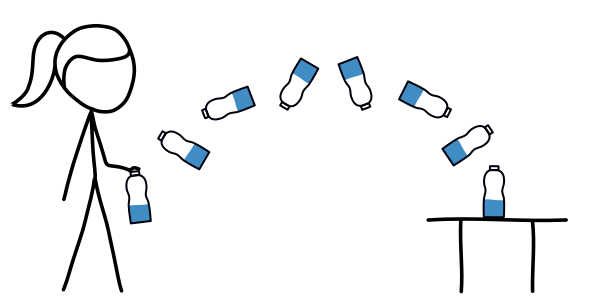
\includegraphics[height=.3\textheight]{sketch}

            \small
            Sketch of a bottle flip. \\
            The bottle is filled to roughly $33\%$, as in Sample Input 1 \\
            ($h = 22$, $r = 4$, $d_a = 1$, $d_w = 4$, optimal height is $7\frac13$).
        \end{column}

        \illustration{.25}{bottles}{Three bottles with different amounts of water.}% Source: Own work
    \end{columns}
\end{frame}
